

% --------------------
\section{Why destructive update matters}
\label{intro:update}

Destructive update is the process of changing the value of an object in-place, by overwriting and hence destroying its old value. Without destructive update we cannot change the values of existing objects, only allocate new ones. 

With deference to Turing completeness, destructive update is \emph{simply not required} to write programs. Likewise, almost every feature of a particular language can be shown to be superfluous. Tiny systems such as the Lambda Calculus, Conway's game of life, and the Rule 30 cellular automata are Turing complete~\cite{rendell:life, cook:universal}, and hence capable of universal computation. On the other hand, no one writes programs in them, at least not directly.

When considering language features we must always start from a practical, and therefore subjective viewpoint. When we say ``destructive update matters", we mean that a large enough subset of programmers find it useful that it warrants consideration by all.

We suggest that destructive update furnishes the programmer with two important and powerful tools, and that these tools are either too cumbersome or too inefficient to create without it. The first tool is a set of efficient array-like data structures for managing collections of objects, and the second is the ability to broadcast a new value to all parts of a program with minimal burden on the programmer.


% --------------------
\subsection{Efficient data structures require destructive update}
For a mechanical device such as an internal combustion engine, efficiency is defined as the ratio of useful work output to the amount of energy input to the device~\cite{giancoli:efficiency}. For a \emph{computational} device such as a collection structure, we could reasonably define its efficiency as being the number of insert and update operations that can be completed per hardware clock cycle. 

We pay no attention to the difficulty of designing the structure in the first place. Like internal combustion engines, the development of common data structures is best left to teams of experts, permitting the end user to focus on their own specific tasks.

When the number of objects to be managed is known beforehand, the simplest collection structure is the array. In a typical garbage collected runtime system, the allocation of an array requires just three machine instructions. We test the top-of-heap pointer to ensure enough space is available, write the object header word, and then advance the pointer. The update of a particular value is also straightforward. Suppose we have three registers: R1 holding a pointer to the array, R2 holding the new value, and R3 holding the index of the value to be updated. Many processors can perform this update with just one or two instructions~\cite{sun:sparc-assembly, intel:instruction-set}.

\begin{center}
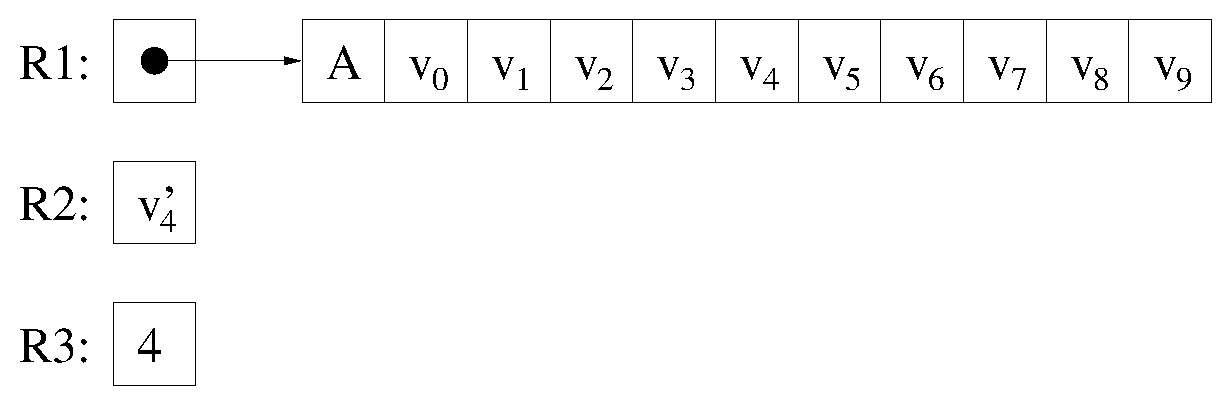
\includegraphics[scale=0.5]{1-Introduction/fig/destructive/data-array10}
\end{center}

Of course, due to pipelining and cache effects, the number of machine instructions executed for an operation does not relate directly to the number of clock cycles used~\cite{hennessy:computer-architecture}. However, it is a usable approximation for this discussion, and we will consider the case of updating a flat array as approaching 100\% efficiency for array-like structures.

Perfect efficiency would be achieved if every update operation completed in the minimum number of clock cycles possible on the available hardware. For most applications, perfect efficiency is unlikely to ever be achieved by a statically compiled program, as it is too difficult to accurately simulate pipeline states and data hazards in a multi-tasking system. 

Ignoring cache effects, the efficiency of an array is independent of how many elements it containts. It costs no more to update a value in a 1000 element array than to update one in a 10 element array.


% --------------------
\subsubsection{Functional arrays are unacceptably slow}
Without destructive update we cannot change an array object once it is allocated, but we can side-step this problem by creating a new object instead of updating the old one. A simple method is to allocate a whole new array and copy the old values into it, with the new value in place of the one that is being updated. This works, but is a disaster for performance. Assuming we need one machine instruction for each value copied, performing an update on a 10 element array now requires 10 instructions, plus three to do the allocation. This represents a miserable 7.7\% efficiency compared with a single instruction destructive update. For a 1000 element array we need at least 1003 instructions, representing approximately 0.1\% efficiency. This is clearly unacceptable.


% --------------------
\subsubsection{Tree structures are only a partial solution}
We can recover some of this ground by using a tree structure instead of a flat array. If we store values in the internal nodes of a balanced binary tree then we need $n$ nodes for $n$ values, and the tree is $\text{ceil} (\log_2(n))$ levels deep. Unfortunately, to change a value in the tree we must still allocate a new node. As this new node will be at a different address from the old one, we must then rebuild all of its parents so that the tree references the new node instead of the old one. For example, in the tree on the next page, to update $v_7$ we must reallocate the node that contains it as well as the nodes of $v_6$, $v_8$ and $v_5$.

\begin{center}
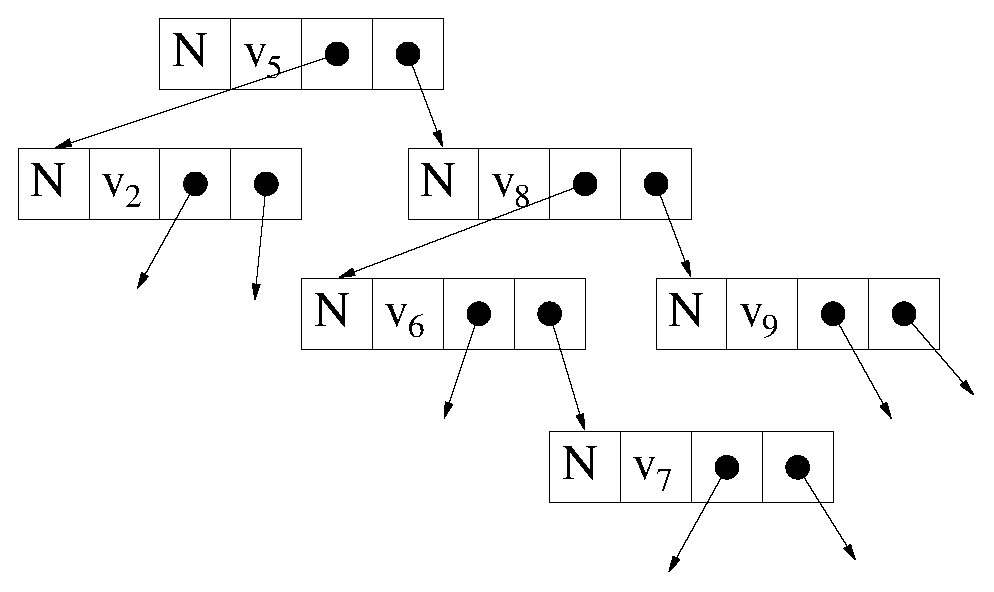
\includegraphics[scale=0.5]{1-Introduction/fig/destructive/data-tree}
\end{center}

For a small number of values, using a binary tree is \emph{worse} than copying the whole array for each update, because each node contains an object header and two pointers instead of just a value. A balanced tree of 1000 elements is 10 levels deep, and as a rough approximation, half of the nodes lie at the bottom of the tree. If we were to update one of these nodes then we would need to reallocate all of its parents, which equates to 9 * 4 = 36 words of space. Not all nodes are at this level, but we haven't accounted for finding the node to be updated in the first place either. For a back-of-envelope calculation we could expect an average of at least 50 machine instructions to be required to update a node in this tree. This equates to 2\% efficiency when compared with destructive array update of a similarly sized array.

Another option is to use trees of a higher order, perhaps a quadtree or a B-tree structure like the one shown in the following diagram. Adding more values per node reduces the depth of the tree. It also reduces the number of nodes we must rebuild when performing an update, but at the cost of making each node larger. 

\begin{center}
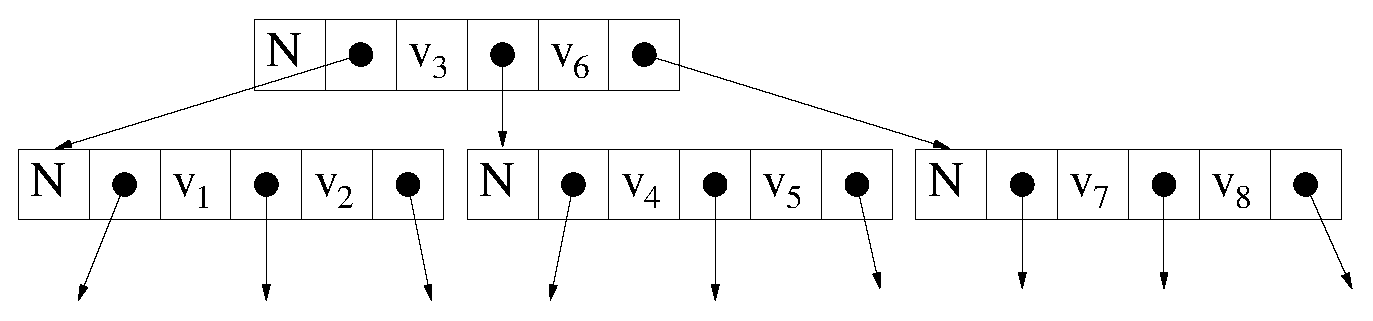
\includegraphics[scale=0.5]{1-Introduction/fig/destructive/data-btree}
\end{center}

For a full (2,3)-tree with two keys and three branches per node, each node is 6 words long including the object header. Every extra level provides three times the number of nodes present in the previous level, and for 1000 values we need a little more than 6 levels. If we say that each node to be updated has an average of 5 parent nodes, this equates to 5 * 6 = 30 words of space to be reinitialised when updating a node. This isn't much better than the previous case.

Many algorithms naturally use an array as their primary collection structure. If, for the lack of destructive update, we are forced to a tree instead, then we automatically impose a $\log(n)$ slowdown on our algorithm's run time. To access an element in a tree we must traverse its structure, but array access can be performed in constant time. This slowdown is in addition to a substantial constant factor due to the extra book-keeping data that must be maintained, such as object headers and branch pointers that are not needed when using arrays. In \cite{ponder:inefficient} Ponder gives a list of algorithms for which no equivalent, array-less algorithm of similar complexity is known. 


% --------------------
\subsubsection{The limit}
There are an infinite variety of possible structures for simulating arrays, and trees represent just a few. By this stage, an astute reader may be thinking about all their own favourite structures and how much better they are than the ones outlined here \cite{okasaki:pure-data, okasaki:intmaps}. As we are talking about machine instructions and constant factors, not just algorithmic complexity, there are also a huge variety of low level details to consider. Details include instruction selection, caching, data layout, pointer compression \cite{lattner:pointer-compression}, and using ``diff arrays'' which rely on destructive update behind the scenes for efficiency, whilst presenting a functionally pure interface. An example of pointer compression is to replace each of the pointers in an object by offsets from a base pointer, instead of including the store address in full. This can result in substantial space savings for pointer heavy programs on 64 bit machines, where the size of a particular data structure is only a tiny fraction of the available address space. Diff arrays use a destructively updateable array for the current state of the structure, and updates to the structure are implemented by physically updating this array. Old states of the array are represented by a list of differences to apply to the current state, so old states become slower and slower to access as the program progresses.

There are many avenues for improvement, but without destructive update we are still hamstrung by the need to allocate objects to represent new program states. Consider a maximally efficient structure which requires only a single, tiny object to be allocated for each update. At the least, we could expect this new object to contain a header word, the new value, and a pointer to the rest of the structure: 

\begin{center}
\includegraphics[scale=0.5]{1-Introduction/fig/destructive/data-tiny}
\end{center}

\vspace{-1em}
However, the allocation and initialisation of this object will still require at least five machine instructions, three for allocation and two to write the new value and pointer. For some applications a constant five-fold slow down is of no consequence, but for others it is a deal breaker. 


\clearpage{}
% --------------------
\subsubsection{Tuples and records are also arrays}

At the machine level, tuples and record objects are often very similar to arrays. We can implement records by representing each field as a pointer to the object containing its value, so at this level the record is simply an array of pointers. A record object with 5 fields would contain a header word and five pointers. Consider then the following record type from DDC:

\begin{lstlisting}
data SquidS 
    = SquidS
    { stateTrace           :: Maybe Handle			
    , stateTraceIndent     :: Int
    , stateErrors          :: [Error]
    , stateStop            :: Bool 
    , stateArgs            :: Set Arg	
    , stateSigmaTable      :: Map Var Var
    , stateVsBoundTopLevel :: Set Var
    , stateVarGen          :: Map NameSpace VarBind 
    , stateVarSub          :: Map Var  Var 
    , stateGraph           :: Graph
    , stateDefs            :: Map Var Type
    , statePath            :: [CBind]
    , stateContains        :: Map CBind (Set CBind)
    , stateInstantiates	   :: Map CBind (Set CBind)
    , stateGenSusp         :: Set Var
    , stateGenDone         :: Set Var
    , stateInst            :: Map Var (InstanceInfo Var Type)			
    , stateQuantifiedVars  :: Map Var (Kind, Maybe Type)
    , stateDataFields      :: Map Var ([Var], [(Var, Type)]) 
    , stateProject         :: Map Var (Type, Map Var Var)	
    , stateProjectResolve  :: Map Var Var
    , stateClassInst       :: Map Var [Fetter] }
\end{lstlisting}

This record represents the state of our type inferencer while it is reducing constraints. The meaning of the fields is not important for this discussion. We include this data type to make the point that real records can contain upwards of 22 separate fields. No matter how efficiently the internal sets, maps and graphs are implemented, without destructive update we cannot change the value of a field without rebuilding at least part of the record object. If we must rebuild it all, then this is at least 22 times slower than using destructive update.

In a language without destructive update we must allocate and initialize new objects to represent new program states. This a drastically less efficient alternative. In practice, even if a language does not support the destructive update of arbitrary structures, attempts are made to introduce it in a more restricted form. In \cite{sastry:order-of-evaluation-analysis} Sastry presents an analysis to determine an order of evaluation for array access and update operations, that allows the updates to be implemented destructively. Besides being first order only, the trouble with many such analyses is that when they fail to introduce an update at an important point in the program, the programmer is left with little recourse to add it manually. There is also the problem of determining which updates \emph{should} have been implemented destructively, but weren't. 

As discussed in \S\ref{intro:monads}, Haskell includes a monadic sub-language that supports the destructive update of select structures such as arrays. However, this sub-language introduces its own problems, and algebraic data such as records and lists cannot be similarly updated. In \cite{sansom:time-profiling} Sansom describes the time profile of an early version of GHC, and mentions that the use of a monadic mutable array over an association list improved the performance of type substitution by a factor of 10. When combined with other improvements, this resulted in a 20x speedup of the type checker as a whole.
 
If a particular programmer does not use functional arrays or large records in their programs, then they may not be aware of the run-time cost of using them. However, those who do are looking down the barrel of a five fold slow-down, or worse, compared with other languages.


% --------------------
\subsection{Destructive update helps to broadcast new values}
\label{Intro:Update:broadcast}
There is an often rehearsed argument that the expressiveness of a language is more important than efficiency, because improvements to processor speed will quickly recover any lost ground. The standard counter is to say that the common man wants their new and faster computers to do \emph{new and faster things}, not the original things less efficiently.

These arguments can also be applied to destructive update. ``Surely'', the antagonist offers, ``a five fold slow-down is not \emph{that} bad. Moore's law says we'll have that back in four years, and look at all the extra compiler optimisations we can do now that the language is pure!''.

Computational efficiency may or may not matter to a particular programmer, but the level of abstraction offered by the language should matter to all. We will now move away from concerns over run time speed, and instead focus on the expressiveness of the language itself. Consider a set of program modules which all reference a single, shared value. This value could be a cursor position or timing value, something that changes often and is of interest to many separate modules. We will refer to this value as X. In a language with destructive update we can place X in a container structure and have each module access it via a pointer:

\begin{center}
\includegraphics[scale=0.6]{1-Introduction/fig/destructive/broadcast-direct}
\end{center}

Using destructive update, one module can modify X and the new version is immediately visible to others. Notice that module 1 has a reference to the top of the container structure as well as a description of how to find the value of interest. In this example the container is a binary tree and the value is accessable by following three right branches from the root node. On the other side, modules 2, 3, and 4 do not need to know how to locate X within its container because they have a pointer directly to it. This second group of modules is not interested in the container or any other value contained within.

Without destructive update, a module cannot change X directly, nor can it change the pointers within client modules so that they reference any new objects it might create. The programmer is forced to rewrite all modules so that they reference the top level of the container structure, and include a description of how to find the value of interest.

\begin{center}
\includegraphics[scale=0.6]{1-Introduction/fig/destructive/broadcast-toplevel}
\end{center}

By doing this we have reduced the level of abstraction in the program. Whereas modules 2, 3, and 4 are only interested in the value X, they must now also concern themselves with the container structure and how to find and update elements contained within.

This problem is compounded when a shared value is logically part of several containers. Perhaps X is also present in a graph structure, and the tree is used to represent a set of objects which must be written to disk when the program finishes. The modules that wish to update the shared value must have knowledge of all structures which contain it.

Shared values like the one described here are often needed to write interactive programs such as Frag \cite{cheong:frag}. In Haskell, variables holding timing values, mouse positions and other user interface states are typically bundled up into a record of IORefs. This in turn requires all code which accesses these values to be written in the IO monad, a point we will return to in \S\ref{intro:monads}.


% --------------------
\subsubsection{Updating nested records in Haskell is painful}

Haskell 98 has an conspicuously poor record system. In itself this is not a new observation, but we pause to discuss it because we feel the problem arises in part from the lack of destructive update in the ambient language. Standard complaints include the records not being light weight, not being extensible, and that all field names are in the top level scope \cite{peyton-jones:records}. In addition, we consider the syntax for updating nested records to be unusable.
 
The following code defines three record types with two fields each. Type \texttt{R1} contains type \texttt{R2}, and type \texttt{R2} contains type \texttt{R3}. Notice the prefixes \texttt{r1}, \texttt{r2} and \texttt{r3} on each field name. In Haskell, field names pollute the top level name space, so we can't have a field named \texttt{field1} in \texttt{R1} as well as in \texttt{R2} without creating a name clash.

\clearpage{}
\begin{lstlisting}
data R1 = R1 { r1Field1  :: Int
             , r1Field2  :: R2 }

data R2 = R2 { r2Field1  :: Char
             , r2Field2  :: R3 }

data R3 = R3 { r3Field1  :: Bool
             , r3Count   :: Int }
\end{lstlisting}

We will create a record value of type \texttt{R1} as an example. Similarly to the previous section, we treat the field \texttt{r3Count} as a shared value that many program modules will be interested in. When the record is created we will initialise this field to zero. The exact values used for the other fields are not important for this example.

\begin{lstlisting}
record1 = R1 { r1Field1 = 5
             , r1Field2 = 
                  R2 { r2Field1 = 'a'
                     , r2Field2 =
                          R3 { r3Field1 = False
                             , r3Count  = 0 }}}
\end{lstlisting}

Extracting the counter field from the structure is straightforward. Each field name becomes a projection function which takes the record and produces the field value, for example \texttt{r1Field1 :: R1 -> Int}. We can make use of the function composition operator to extract the count field using a pleasing syntax:

\begin{lstlisting}
count  = (r3Count . r2Field2 . r1Field2) record1
\end{lstlisting}

Updating the counter is another matter entirely. As we do not wish to modify the other fields in the structure, we must unpack and repack each level in turn. This process corresponds to reallocating parents when updating a node in a tree. Unfortunately, this time we cannot write a cute recursive function to do so because the records at each level have different types. The following diagram shows the structure of the nested records:

\begin{center}
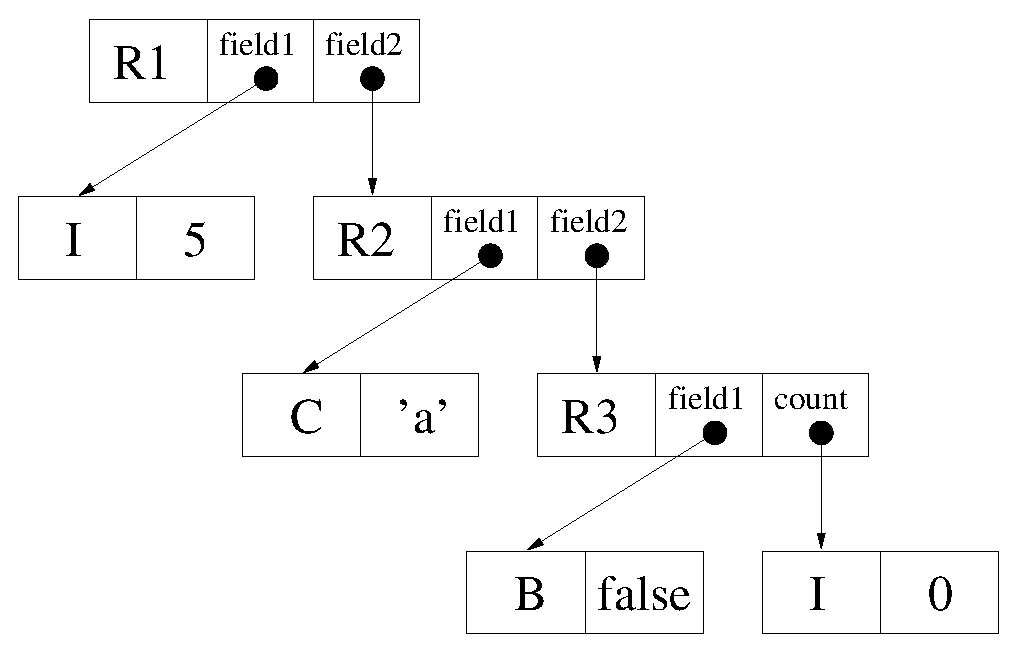
\includegraphics[scale=0.5]{1-Introduction/fig/destructive/broadcast-record}
\end{center}

\clearpage{}
\begin{center}
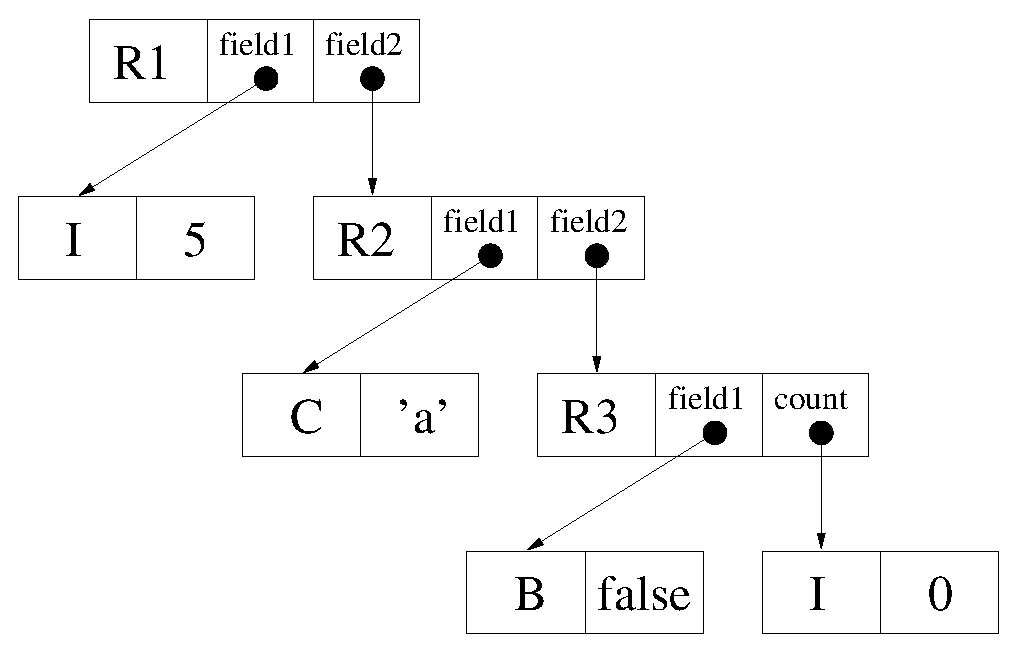
\includegraphics[scale=0.5]{1-Introduction/fig/destructive/broadcast-record}
\end{center}

If we wish to change the \emph{count} field in this structure to the value 1, we must allocate a new object containing this value. We must then rebuild the \texttt{R3}, \texttt{R2} and \texttt{R1} nodes so that the structure references this new object while retaining the pointers to the other nodes. Here is the gory Haskell expression:

\begin{lstlisting}
record2
  = record1 { r1Field2 = 
      (r1Field2 record1) { r2Field2 = 
         ((r2Field2 . r1Field2) record1) { r3Count = 1 }}}
\end{lstlisting}

Clearly this is not something a typical programmer would enjoy writing. The field names and the variable \texttt{record1} are repeated twice each, the line must be broken into fragments to fit on the page, it does not indent well, and there is much visual noise.

It is worse when we need to update this field with a non-trivial expression. Consider the simple act of incrementing \texttt{r3Count}. We can use layout to reduce the noise, but it is still quite bad:
\begin{lstlisting}
record3
  = record2 { 
      r1Field2 = (r1Field2 record2) {
      r2Field2 = ((r2Field2 . r1Field2) record2) {
      r3Count  = (r3Count . r2Field2 . r1Field2) record2 + 1 
    }}}
\end{lstlisting}
The need to write such tedious code to perform such a simple update would be a deal breaker for many programmers.\footnote{It certainly is for the author.}

Consider an equivalent statement in an imperative language, such as C++.
\begin{lstlisting}
record2.field2.field2.count += 1
\end{lstlisting}
Destructive update allows the programmer to focus solely on the element of interest, while leaving the others untouched. Granted, the above statement does not have the same semantics as the Haskell version because it modifies the original object instead creating a new one. If this behaviour is required then many imperative, object oriented languages support a fragment such as:
\begin{lstlisting}
record3 = record2.copy()
record3.field2.field2.count += 1
\end{lstlisting}
To the surrounding program these two simple statements have the same effect as the Haskell expression shown above, with the added advantage that the concepts of \emph{copy} and \emph{update} are clearly separated.

In C++ we can make life even easier for the programmer. We can create a reference to the field of interest and increment it without any knowledge of the surrounding record structure:
\begin{lstlisting}
int* countRef = &(record.field2.field2.count)

(*countRef) += 1;
\end{lstlisting}

Admittedly, references and destructive update can be used for evil as well as for good. Many confusing programs can be constructed in which different program modules communicate via shared mutable objects in a way which is entirely non-obvious to the casual observer, and almost impossible to debug. The counter to this argument is to say that confusing programs can be written in any language, and a good carpenter can hammer a nail into a wall without smashing their own fingers.

We should note that the problem of updating nested records in Haskell can be made easier by generic programming libraries such as `Scrap Your Boilerplate'~\cite{lammel:scrap-your-boilerplate} (SYB) and DriFT~\cite{hinze:generic-programming-in-haskell}. Although these systems can help, we feel they are not complete solutions as they lack the efficiency and ease of use of destructive update. SYB style systems tend to traverse uninteresting parts of a structure when performing an update, resulting in a significant performance penalty~\cite{mitchell:neil}. DriFT is a preprocessor which can automatically generate update functions for each of the fields in a record, though it does not support nested update as per the previous example. When implementing DDC we defined tuples of get and set functions for each field, along with combinators to compose these functions and to update fields deep within nested records. We have found this to be a serviceable yet tedious approach, as we have not yet written a preprocessor to generate the tuples. This approach also does not solve the problem of field names being in top level scope.

